%
% Complete documentation on the extended LaTeX markup used for Insight
% documentation is available in ``Documenting Insight'', which is part
% of the standard documentation for Insight.  It may be found online
% at:
%
%     http://www.itk.org/

\documentclass{InsightArticle}

\usepackage[dvips]{graphicx}

%%%%%%%%%%%%%%%%%%%%%%%%%%%%%%%%%%%%%%%%%%%%%%%%%%%%%%%%%%%%%%%%%%
%
%  hyperref should be the last package to be loaded.
%
%%%%%%%%%%%%%%%%%%%%%%%%%%%%%%%%%%%%%%%%%%%%%%%%%%%%%%%%%%%%%%%%%%
\usepackage{amsmath}
\usepackage{amssymb}
\usepackage{amsthm}
\usepackage{subfigure}
\usepackage{float}

\usepackage[dvips,
pagebackref=true,
pdfhighlight=/I,
bookmarks=true,
bookmarksopen=true,
% backref=true,
colorlinks=true,
linkcolor=blue,
citecolor=blue,
urlcolor=blue,
pdfauthor={A. Gelas, A. Gouaillard and S. Megason}
pdftitle={Surface Mesh Discrete Curvature Estimators},
pdfcenterwindow=true,
pdffitwindow=true,
hyperfigures=true
]{hyperref}
% \usepackage{algorithm}
% \usepackage{algpseudocode}
\graphicspath{{fig/}}




\def \Surface {\mathcal{S}}
\def \Rset {\mathbb{R}}
\def \ie {\textit{i.e. }}
\def \etal {\textit{et al. }}


\theoremstyle{plain}
\newtheorem*{note}{Note}

%  This is a template for Papers to the Insight Journal.
%  It is comparable to a technical report format.

% The title should be descriptive enough for people to be able to find
% the relevant document.
\title{Surface Mesh Discrete Curvature Estimators}

% Increment the release number whenever significant changes are made.
% The author and/or editor can define 'significant' however they like.
\release{0.01}

% At minimum, give your name and an email address.  You can include a
% snail-mail address if you like.
\author{Arnaud Gelas, Alexandre Gouaillard\\
and Sean Megason}
\authoraddress{Department of System Biology, Harvard Medical School,\\
Boston, MA 02115, USA}

\begin{document}


\ifpdf
\else
   %
   % Commands for including Graphics when using latex
   %
   \DeclareGraphicsExtensions{.eps,.jpg,.gif,.tiff,.bmp,.png}
   \DeclareGraphicsRule{.jpg}{eps}{.jpg.bb}{`convert #1 eps:-}
   \DeclareGraphicsRule{.gif}{eps}{.gif.bb}{`convert #1 eps:-}
   \DeclareGraphicsRule{.tiff}{eps}{.tiff.bb}{`convert #1 eps:-}
   \DeclareGraphicsRule{.bmp}{eps}{.bmp.bb}{`convert #1 eps:-}
   \DeclareGraphicsRule{.png}{eps}{.png.bb}{`convert #1 eps:-}
\fi


\maketitle


\ifhtml
\chapter*{Front Matter\label{front}}
\fi


% The abstract should be a paragraph or two long, and describe the
% scope of the document.
\begin{abstract}
\noindent Computing local curvatures of a given surface is important for applications, shape analysis, surface segmentation, meshing, and surface evolution. For a given smooth surface (with a given analytical expression which is sufficiently differentiable) curvatures can be analytically and directly computed. However in real applications, one often deals with a surface mesh which is an insufficiently differentiable approximation, and thus curvatures must be estimated. Based on a surface mesh data structure (\code{itk::QuadEdgeMesh}~\cite{itkQE}), we introduce and implement curvature estimators following the approach of Meyer\etal\cite{Meyer02}. We show on a sphere that this method results in more stable curvature approximations than the commonly used discrete estimators (as used in VTK: \code{vtkCurvatures}).
\end{abstract}

\tableofcontents

%%%%%%%%%%%%%%%%%%%%%%%%%%%%%%%%%%%%%%%%%
\section{Introduction}

Local curvatures provide information about the local behavior of the surface in vicinity of a given point, and so play an important role when working with surfaces. For example, the Gaussian curvature gives information about the location of the surface with the tangent plane at the considered point; a positive value means that the surface is locally either a peak or a valley; a negative value means that the surface is locally a saddle; a null value means the surface is locally flat in at least one direction (planar or cylindrical). The computation of local curvatures is a necessary step in many applications such as shape analysis, surface segmentation, adaptive surface meshing, remeshing, and surface evolution with active contours.

Unfortunately local curvatures are only defined for smooth surfaces, and when dealing with surface meshes only estimators are available. Over the last decade, many estimators have been proposed in the literature~\cite{MeshCourse07}. Here we first introduce differential properties of 2-manifold smooth surfaces (in section~\ref{sec:Background:Smooth}), then we present discrete estimators from~\cite{Meyer02} that we implemented (in section~\ref{sec:Background:Discrete}) and provide information about their use in an application (see section~\ref{sec:Implementation}-\ref{sec:Usage}). Finally in section~\ref{sec:Results}, we test our method on a sphere mesh and compare our results with the theoretical ones and with the usual discrete estimators (as it is used in VTK: \code{vtkCurvatures}).

%%%%%%%%%%%%%%%%%%%%%%%%%%%%%%%%%%%%%%%%%
\section{Background}
\label{sec:Background}

Taken from~\cite{MeshCourse07}, we first introduce differential properties of 2-manifold surfaces and then give details from the discrete curvature estimators from~\cite{Meyer02}.

%%%%%%%%%%%%%%%%%%%%%%%%%%%%%%%%%%%%%%%%%
\subsection{Differential Geometry}
\label{sec:Background:Smooth}

Consider a continuous surface $\Surface \subset \Rset^3$ given in a parametric form as

\begin{equation}
  \mathbf{x}(u,v)=
\left(
  \begin{array}{c}
    x(u,v)\\
    y(u,v)\\
    z(u,v)
  \end{array}
\right),\ (u,v)\in \Rset^2
\end{equation}
where $x$, $y$, $z$ are differentiable functions in $u$ and $v$. The partial derivatives $\mathbf{x}_u$ and $\mathbf{x}_v$ span the tangent plane to $\Surface$ at a given location $\mathbf{p}$. Assuming a regular parametrization ($\mathbf{x}_u \times \mathbf{x}_v$), the normal vector is then given as $\mathbf{n} = \mathbf{x}_u \times \mathbf{x}_v / \left\| \mathbf{x}_u \times \mathbf{x}_v \right\|$.

%%%%%%%%%%%%%%%%%%%%%%%%%%%%%%%%%%%%%%%%%
\subsubsection{First Fundamental form}
The \emph{first fundamental form} of $\mathbf{x}$ is given by the matrix
\begin{equation}
  \mathbf{I} =
\left[
  \begin{array}{cc}
    E & F \\
    F & G
  \end{array}
\right] =
\left[
  \begin{array}{cc}
    \mathbf{x}_u^T \mathbf{x}_u & \mathbf{x}_u^T \mathbf{x}_v\\
    \mathbf{x}_u^T \mathbf{x}_v & \mathbf{x}_v^T \mathbf{x}_v
  \end{array}
\right]
\end{equation}
which defines an inner product on the tangent space of $\Surface$.

%%%%%%%%%%%%%%%%%%%%%%%%%%%%%%%%%%%%%%%%%
\subsubsection{Second Fundamental form}
The \emph{second fundamental form} is defined as
\begin{equation}
  \mathbf{II} =
\left[
  \begin{array}{cc}
    e & f\\
    f & g
  \end{array}
\right] =
\left[
  \begin{array}{cc}
    \mathbf{x}_{uu}^T \mathbf{n} & \mathbf{x}_{uv}^T \mathbf{n}\\
    \mathbf{x}_{uv}^T \mathbf{n} & \mathbf{x}_{vv}^T \mathbf{n}
  \end{array}
  \right]
\end{equation}
Alternatively, $\mathbf{II}$ can be expressed using the identities $\mathbf{x}_{uu}^T \mathbf{n} = - \mathbf{x}_{u}^T \mathbf{n}_u$, $\mathbf{x}_{uv}^T \mathbf{n} = \mathbf{x}_{vu}^T \mathbf{n} = - \frac{1}{2} \left( \mathbf{x}_{u}^T \mathbf{n}_v + \mathbf{x}_{v}^T \mathbf{n}_u \right)$.

The symmetric bilinear first and second fundamental forms allows the length, angles, area, and curvatures on the surface to be measured.

%%%%%%%%%%%%%%%%%%%%%%%%%%%%%%%%%%%%%%%%%
\subsubsection{Normal Curvature}
Let $\mathbf{t}=a\mathbf{x}_u +b\mathbf{x}_v$ be a unit vector in the tangent plane at $\mathbf{p}$, represented as $\bar{\mathbf{t}}=(a,b)^T$ in the local coordinate system. The \emph{normal curvature} $\kappa_n(\bar{\mathbf{t}})$ is the curvature of the planar curve that results from intersecting $\Surface$ with the plane through $\mathbf{p}$ spanned by $\mathbf{n}$ and $\mathbf{t}$. The normal curvature in direction $\bar{\mathbf{t}}$ can be expressed in terms of the fundamental forms as
\begin{equation}
  \kappa_n(\bar{\mathbf{t}}) = \frac{\bar{\mathbf{t}}^T\cdot\mathbf{II}\cdot \bar{\mathbf{t}}}{\bar{\mathbf{t}}^T\cdot\mathbf{I}\cdot\bar{\mathbf{t}}} =
    \frac{e\ a^2+2f\ ab+ g\ b^2}{E\ a^2+ 2F\ ab+G\ b^2}
\end{equation}

%%%%%%%%%%%%%%%%%%%%%%%%%%%%%%%%%%%%%%%%%
\subsubsection{Curvature Tensor}
The minimal normal curvature $\kappa_1$ and the maximal normal curvature $\kappa_2$ are called the \emph{principal curvatures}. The associated tangent vectors $\mathbf{t}_1$ and $\mathbf{t}_2$ are called \emph{principal directions} and are always perpendicular to each other.

The principal curvatures are also obtained as eigenvalues of the \emph{Weingarten curvature matrix} (or second fundamental tensor)
\begin{equation}
  \mathbf{W} = \frac{1}{EG-F^2}
\left[
  \begin{array}{cc}
    eG-fF & fG-gF\\
    fE-eF & gE-fF
  \end{array}
\right]
\end{equation}

$\mathbf{W}$ represents the Weingarten map or shape operator, which measures the directional derivative of the normal, \ie $\mathbf{W\bar{t}} = \frac{\partial \mathbf{n}}{\mathbf{\bar{t}}}$. This allows the normal curvature to be expressed as
\begin{equation*}
  \kappa_n(\mathbf{\bar{t}}) = \mathbf{\bar{t}}^T\cdot\ \mathbf{W}\cdot\ \mathbf{\bar{t}}
\end{equation*}
With a local coordinate system defined by the principal directions $\mathbf{t}_1$ and $\mathbf{t}_2$, $\mathbf{W}$ is a diagonal matrix:
\begin{equation}
  \mathbf{W} =
\left[
  \begin{array}{cc}
  \mathbf{\bar{t}}_1 & \mathbf{\bar{t}}_2
  \end{array}
\right]
\left[
  \begin{array}{cc}
  \kappa_1 & 0\\
  0 & \kappa_2
  \end{array}
\right]
\left[
  \begin{array}{c}
    \mathbf{\bar{t}}_1\\
    \mathbf{\bar{t}}_2
  \end{array}
\right]
\end{equation}
Then the normal curvature can also be written as
\begin{equation}
  \kappa_n(\mathbf{\bar{t}}) = \kappa_n(\phi) = \kappa_1 \cos^2 \phi + \kappa_2 \sin^2 \phi
\end{equation}
where $\phi$ is the angle between $\mathbf{\bar{t}}$ and $\mathbf{\bar{t}}_1$.

The \emph{curvature tensor} $\mathbf{T}$ is expressed as a symmetric $3\times 3$ matrix with the eigenvalues $\kappa_1, \kappa_2, 0$ and the corresponding eigenvectors $\mathbf{t}_1, \mathbf{t}_2, \mathbf{n}$. The tensor $\mathbf{T}$ measures the change of the unit normal with respect to a tangent vector $\mathbf{t}$ independently of the parametrization. It can be constructed as
\begin{equation}
  \mathbf{T} = \mathbf{P}\cdot\ \mathbf{D}\cdot\ \mathbf{P}^{-1}
\end{equation}
with $\mathbf{P}=\left[\mathbf{t}_1, \mathbf{t}_2, \mathbf{n}\right]$ and $\mathbf{D}=\text{diag}(\kappa_1, \kappa_2, 0)$.

%%%%%%%%%%%%%%%%%%%%%%%%%%%%%%%%%%%%%%%%%
\subsubsection{Gaussian Curvature}
The \emph{Gaussian curvature} $K$ is defined as the product of the principal curvatures
\begin{equation}
  K = \kappa_1\cdot \kappa_2 = \text{det}(\mathbf{W}) \label{eq:GaussCurvatureDef1}
\end{equation}
Gaussian curvature can also be expressed as
\begin{equation}
  K = \lim_{diam(\mathcal{A})\rightarrow 0} \frac{\mathcal{A}^{\mathcal{G}}}{\mathcal{A}}
\end{equation}
where $\mathcal{A}^{\mathcal{G}}$ is the area of the image of the Gauss map (also called the spherical image) associated with infinitesimal surface $\mathcal{A}$.

%%%%%%%%%%%%%%%%%%%%%%%%%%%%%%%%%%%%%%%%%
\subsubsection{Mean Curvature}
The \emph{mean curvature} $H$ is defined as the average of the principal curvatures
\begin{equation}
  H = \frac{\kappa_1 + \kappa_2}{2} = \frac{1}{2} \text{trace}(\mathbf{W}) \label{eq:MeanCurvatureDef1}
\end{equation}
or can alternatively be defined as the continuous average of the normal curvatures
\begin{equation}
  H = \frac{1}{2\pi}\ \int_{0}^{2\pi} \kappa_n(\phi)\ d\phi
\end{equation}

Lagrange noticed that $H=0$ is the Euler-Lagrange equation for surface area minimization. This provides a direct link between surface area minimization and mean area curvature flow:
\begin{equation}
  2 H \cdot \mathbf{n} = \lim_{diam(\mathcal{A})\rightarrow 0} \frac{\nabla \mathcal{A}}{\mathcal{A}}
\end{equation}
where $\mathcal{A}$ is an infinitesimal area around a point $\mathbf{p}$ on the surface, $diam(\mathcal{A})$ its diameter.
%%%%%%%%%%%%%%%%%%%%%%%%%%%%%%%%%%%%%%%%%
\subsection{Discrete Differential Operators}
\label{sec:Background:Discrete}

The differential properties defined in the previous sections require a surface to be sufficiently differentiable, at least it requires the existence of the second derivatives. Since polygonal meshes are piecewise linear surface, the concepts introduced above cannot be applied directly. Thus these differential properties of the underlying surface must be approximated from the mesh data. Several approaches have been proposed in recent years (see~\cite{MeshCourse07}), and here we only describe the ones proposed by Meyer~\textit{et~al.}~\cite{Meyer02}.

%%%%%%%%%%%%%%%%%%%%%%%%%%%%%%%%%%%%%%%%%
\subsubsection{Discrete Gaussian Curvature}

Meyer~\textit{et~al.}~\cite{Meyer02} express the discrete Gaussian curvature as:
\begin{equation}
  K(\mathbf{p}_i) = \frac{2\pi - \sum\limits_{j=1}^{\#f}\theta_j}{\mathcal{A}_{\text{\tiny{Mixed}}}} \label{eq:DiscreteGaussianCurvature}
\end{equation}
where $\theta_j$ is the angle of the $j$-th face at the vertex $\mathbf{p}$ (see Figure~\ref{fig:gauss_angle}), $\#f$ denotes the number of faces around this vertex, and $\mathcal{A}_{\text{\tiny{Mixed}}}$ is the area of the region of influence of a vertex (see the corresponding paragraph below).

\begin{figure}[ht]
  \centering
  \subfigure[]{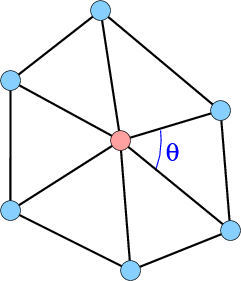
\includegraphics[width=0.2\textwidth]{gauss_angle}\label{fig:gauss_angle}}
  \hspace{0.5cm}
  \subfigure[]{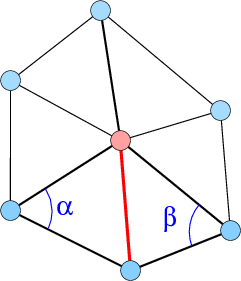
\includegraphics[width=0.2\textwidth]{mean_angle}\label{fig:mean_angle}}
  \caption{$\theta$ is the angle of one face at a vertex $\mathbf{p}$ used for computation of the discrete Gaussian curvature~(a). $\alpha$ and $\beta$ are the opposite angles to a given edge (here in red) used for computing the discrete mean curvature~(b).}
\end{figure}


%%%%%%%%%%%%%%%%%%%%%%%%%%%%%%%%%%%%%%%%%
\subsubsection{Discrete Mean Curvature}

Following~\cite{Meyer02} the mean curvature can be approximated by
\begin{equation}
  H(\mathbf{p}_i) = \frac{1}{4 \mathcal{A}_{\text{\tiny{Mixed}}}} \left\| \sum_{j \in N(i)} \left( \cot \alpha_{ij} + \cot \beta_{ij} \right) ( \mathbf{p}_i - \mathbf{p}_j ) \right\| \label{eq:DiscreteMeanCurvature}
\end{equation}
where $\alpha_{ij}$ and $\beta_{ij}$ are the angle opposite to the edge $\mathbf{p}_i\mathbf{p}_j$ (see Figure~\ref{fig:mean_angle}), $N(i)$ is the set of vertices in the 0-ring of $\mathbf{p}_i$, $\mathcal{A}_{\text{\tiny{Mixed}}}$ is the area of the region of influence of a vertex (see the corresponding paragraph below).

%%%%%%%%%%%%%%%%%%%%%%%%%%%%%%%%%%%%%%%%%
\subsubsection{Region of influence}
\label{sec:RegionOfInfluence}

The \emph{region of influence} of a given vertex does not overlap with any other region of influence, and represents a local part of the surface on the vicinity of $\mathbf{p}$. Following the definition of Meyer~\textit{et~al.}~\cite{Meyer02}, there are 3 different configurations for its computation (see Figure~\ref{fig:mixed_area}), and thus the computation of its area follows the algorithm:
\begin{itemize}
  \item $\mathcal{A}_{\text{\tiny{Mixed}}} = 0$
  \item For each triangle $T$ from the 1-ring neighborhood of $\mathbf{p}$
    \begin{itemize}
      \item If $T$ is non-obtuse (Voronoi safe)\\
        $\mathcal{A}_{\text{\tiny{Mixed}}}$ += Voronoi region of $\mathbf{p}$ in $T$
      \item Else
        \begin{itemize}
          \item If the angle of $T$ at $\mathbf{p}$ is obtuse\\
            $\mathcal{A}_{\text{\tiny{Mixed}}}$ += area(T) / 2
          \item Else\\
            $\mathcal{A}_{\text{\tiny{Mixed}}}$ += area(T) / 4
        \end{itemize}

    \end{itemize}

\end{itemize}


\begin{figure}[htbp]
  \centering
  \subfigure[]{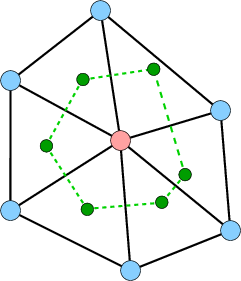
\includegraphics[width=0.2\textwidth]{mixed_area0}\label{fig:mixed_area0}}
  \hspace{0.5cm}
  \subfigure[]{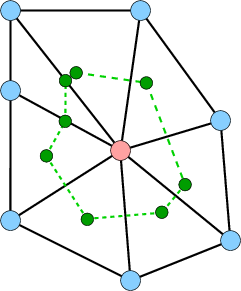
\includegraphics[width=0.2\textwidth]{mixed_area2}\label{fig:mixed_area2}}
  \hspace{0.5cm}
  \subfigure[]{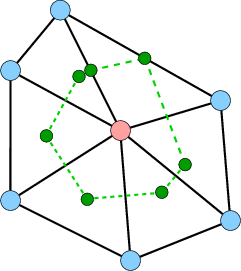
\includegraphics[width=0.2\textwidth]{mixed_area1}\label{fig:mixed_area1}}
  \caption{Here we show the 3 different configurations for the region of influence of a given vertex $\mathbf{p}$. The region of influence is delimited by the green lines, and its area is $\mathcal{A}_{\text{\tiny{Mixed}}}$. All triangles are non-obtuse and the region of influence is identical to the Voronoi region~(a). If there is one obtuse triangle, the influence region is then composed of Voronoi region for each non-obtuse triangle, then for the obtuse ones the corresponding region differs if the angle at the vertex $\mathbf{p}$ is obtuse~(b) or not~(c).}
  \label{fig:mixed_area}
\end{figure}

%%%%%%%%%%%%%%%%%%%%%%%%%%%%%%%%%%%%%%%%%
\subsubsection{Principal Curvatures}
From Eq.~\ref{eq:GaussCurvatureDef1}-~\ref{eq:MeanCurvatureDef1}, the principal curvatures can then be computed as
\begin{eqnarray}
  \kappa_1( \mathbf{p} ) = H( \mathbf{p} ) + \sqrt{\Delta( \mathbf{p} )}\\
  \kappa_2( \mathbf{p} ) = H( \mathbf{p} ) - \sqrt{\Delta( \mathbf{p} )}
\end{eqnarray}
where $\Delta( \mathbf{p} ) = H^2( \mathbf{p} ) - G( \mathbf{p} )$, $G( \mathbf{p} )$ is given by Eq.~\ref{eq:DiscreteGaussianCurvature} and $H( \mathbf{p} )$ by Eq.~\ref{eq:DiscreteMeanCurvature}.

While the continuous case $\Delta$ is always positive, in the discrete case we must ensure that it is, by thresholding it to zero (even if it occurs rarely).

%%%%%%%%%%%%%%%%%%%%%%%%%%%%%%%%%%%%%%%%%
% \subsubsection{Principal Directions}

%%%%%%%%%%%%%%%%%%%%%%%%%%%%%%%%%%%%%%%%%
\section{Implementation}
\label{sec:Implementation}

We provide implementations of the previous discrete curvature estimators, \ie
\begin{itemize}
  \item Gaussian curvature (\code{itk::QEMeshDiscreteGaussianCurvatureEstimator}),
  \item mean curvature (\code{itk::QEMeshDiscreteMeanCurvatureEstimator}),
  \item minimal curvature (\code{itk::QEMeshDiscreteMinCurvatureEstimator}),
  \item maximal curvature (\code{itk::QEMeshDiscreteMaxCurvatureEstimator}).
\end{itemize}

%%%%%%%%%%%%%%%%%%%%%%%%%%%%%%%%%%%%%%%%%
\section{Usage}
\label{sec:Usage}

These 4 filters are used in the same way, and in the following example we assume the user wants to compute the Gaussian curvature of a given mesh. However to compute the mean, minimal or maximal curvature, the user only needs to define the corresponding estimator as the \code{CurvatureFilterType}, see given source code~\code{DiscreteCurvatureEstimator.cxx}.

% \begin{verbatim}
%   typedef itk::QuadEdgeMeshExtendedTraits <
%     CoordType,
%     Dimension,
%     2,
%     CoordType,
%     CoordType,
%     CoordType,
%     bool,
%     bool > Traits;
%
%   typedef itk::QuadEdgeMesh< CoordType, Dimension, Traits > MeshType;
%   typedef itk::QEMeshDiscreteGaussianCurvatureEstimator<MeshType,MeshType>
%     CurvatureFilterType;
%
%   typedef VTKPolyDataReader< MeshType > ReaderType;
%
%   ReaderType::Pointer reader = ReaderType::New( );
%   reader->SetFileName( argv[1] );
%   try
%     {
%     reader->Update( );
%     }
%   catch( itk::ExceptionObject & exp )
%     {
%     std::cerr << "Exception thrown while reading the input file " << std::endl;
%     std::cerr << exp << std::endl;
%     return EXIT_FAILURE;
%     }
%
%   MeshType::Pointer mesh = reader->GetOutput();
%
%   CurvatureFilterType::Pointer gaussian_curvature = CurvatureFilterType::New();
%   gaussian_curvature->SetInput( mesh );
%   gaussian_curvature->Update();
%
%   MeshType::Pointer output = gaussian_curvature->GetOutput();
% \end{verbatim}
%
\begin{note}
If the connectivity of the starting mesh is not important, we recommend prefiltering the mesh through a Delaunay conforming filter (\code{itk::DelaunayConform}~\cite{itkDelaunayConform}) to improve the accuracy of curvature approximations.
\end{note}

%%%%%%%%%%%%%%%%%%%%%%%%%%%%%%%%%%%%%%%%%
\section{Results}
\label{sec:Results}

To validate our implementations, we estimate curvatures on a sphere of radius $0.5$. All the curvatures are known for the smooth surface and thus we can easily compare the theoretical values to the experimental ones (see Figure~\ref{fig:our_sphere_curv}).

\begin{itemize}
  \item Gaussian curvature $K$ is supposed to be 4 at any point of the sphere. In practice with our filter, we get $4$ with a maximal error below $1\%$ (see Figure~\ref{fig:sphere_gauss_curvature}).
  \item mean curvature $H$ is supposed to be 2 at any point of the sphere. In practice with our filter, we get $2$ with a maximal error below $1\%$ (see Figure~\ref{fig:sphere_mean_curvature}).
  \item $\Delta = H^2 - K$ is supposed to be 0 at any point of the sphere. In practice some negative value occurs, and there the maximum error is about $1\%$ (see Figure~\ref{fig:sphere_delta_no_threshold}).
  \item min curvature $\kappa_1$ is supposed to be 2 at any point of the sphere. In pratice with our filter, we get $2$ with a maximal error error $7\%$ (see Figure~\ref{fig:sphere_min_curvature}).
  \item max curvature $\kappa_2=2$ is supposed to be 2 at any point of the sphere. In pratice with our filter, we get $2$ with a maximal error error $7\%$ (see Figure~\ref{fig:sphere_max_curvature}).
\end{itemize}


\begin{figure}[tb]
  \centering
  \subfigure[Gaussian $K$]{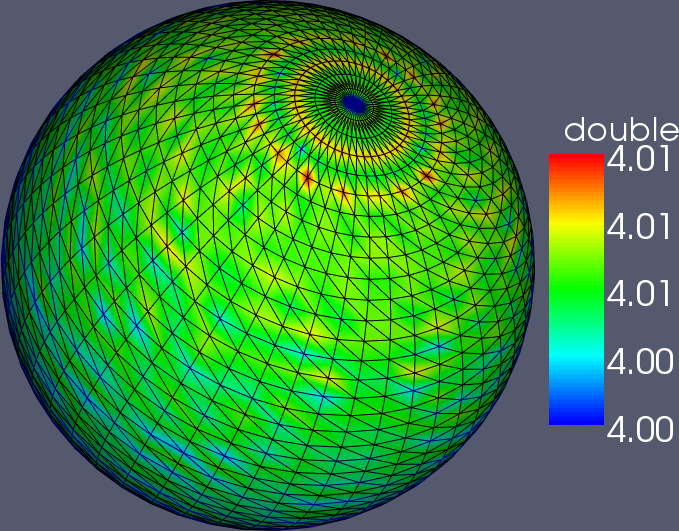
\includegraphics[height=0.19\textheight]{sphere_gauss_curvature}\label{fig:sphere_gauss_curvature}}
  \subfigure[mean $H$]{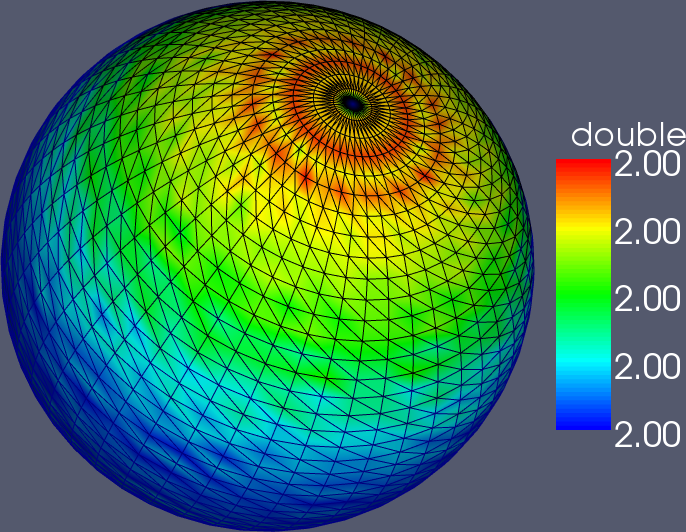
\includegraphics[height=0.19\textheight]{sphere_mean_curvature}\label{fig:sphere_mean_curvature}}
  \subfigure[$H^2-K$]{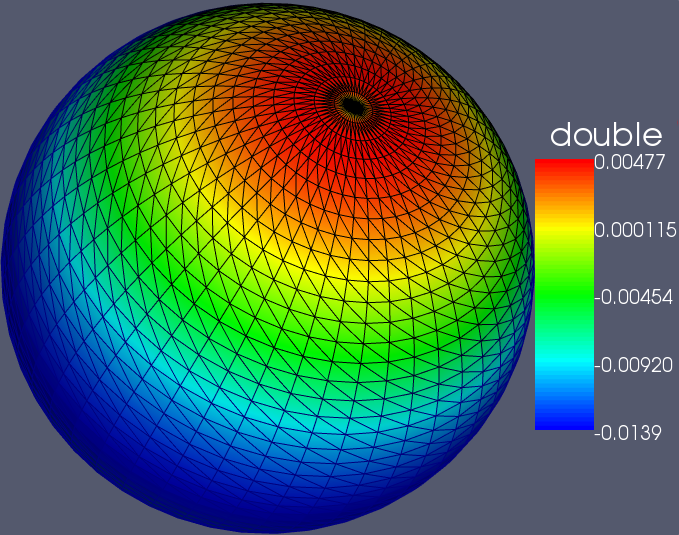
\includegraphics[height=0.19\textheight]{sphere_delta_no_threshold}\label{fig:sphere_delta_no_threshold}}
  \subfigure[$\kappa_1$]{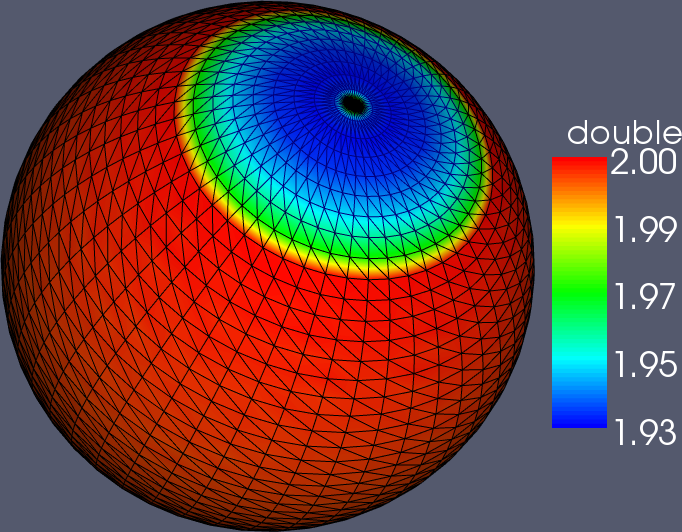
\includegraphics[height=0.19\textheight]{sphere_min_curvature}\label{fig:sphere_min_curvature}}
  \subfigure[$\kappa_2$]{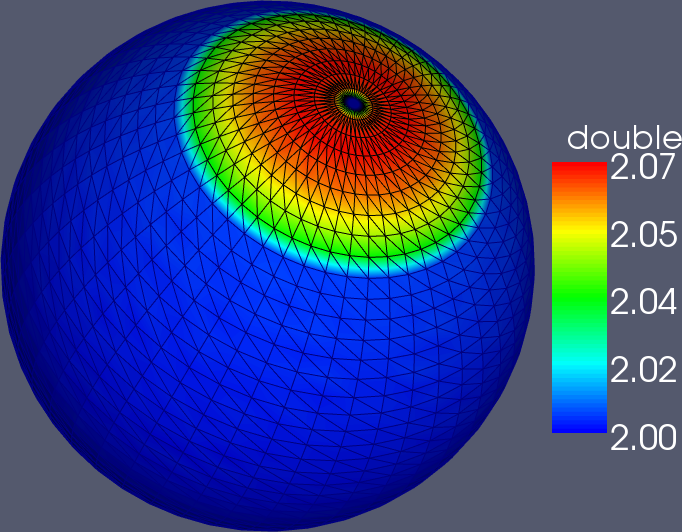
\includegraphics[height=0.19\textheight]{sphere_max_curvature}\label{fig:sphere_max_curvature}}
  \caption{Results using our implementations for discrete curvature estimators on a sphere.} \label{fig:our_sphere_curv}
\end{figure}

Here we compare the results on the sphere of our filter with the one provided in VTK (see Figure~\ref{fig:sphere_gauss_comparison}-\ref{fig:sphere_mean_comparison}). Both estimators provide excellent approximations of curvature where the vertex degree is 6, however vertices with extraordinary degree and really elongated triangles, \ie poles, exhibit an important error when using usual estimators. As claimed by Meyer\etal\cite{Meyer02} their estimators is less dependent to the triangle shape and vertex degree.

\section*{Acknowledgment}
This work was funded by a grant from the NHGRI (P50HG004071-02) to found the Center for in toto genomic analysis of vertebrate development.

%%%%%%%%%%%%%%%%%%%%%%%%%%%%%%%%%%%%%%%%%
%
%  Insert the bibliography using BibTeX
%
%%%%%%%%%%%%%%%%%%%%%%%%%%%%%%%%%%%%%%%%%

\bibliographystyle{plain}
\bibliography{curvature}

\begin{figure}[tb]
  \centering
  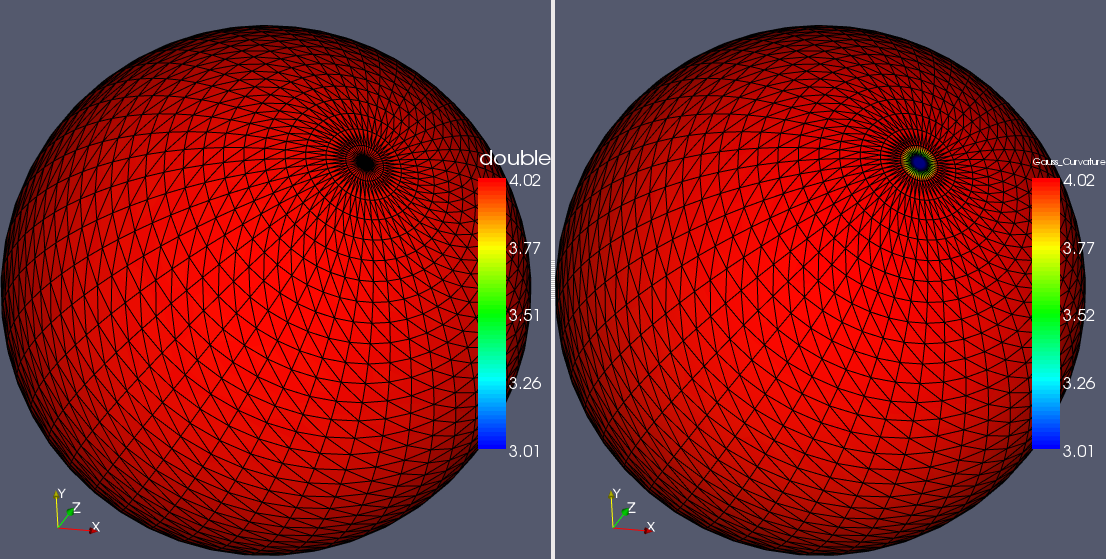
\includegraphics[height=0.2\textheight]{sphere_gauss_curvature_compare}
  \caption{Comparison of our Gaussian curvature estimator on the left and the one provided by VTK.}
  \label{fig:sphere_gauss_comparison}
\end{figure}

\begin{figure}[htbp]
  \centering
  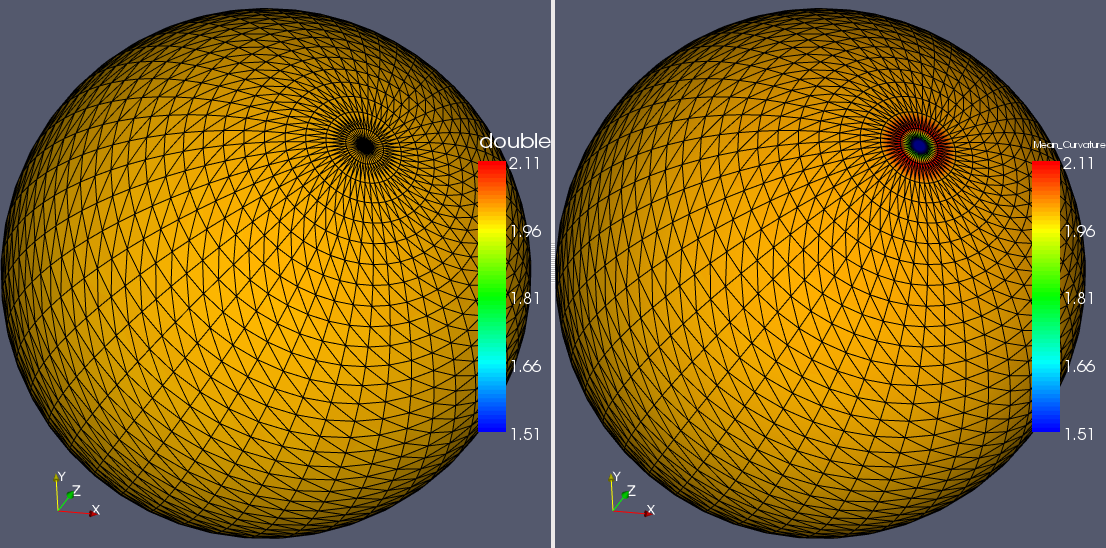
\includegraphics[height=0.2\textheight]{sphere_mean_curvature_compare}
  \caption{Comparison of our mean curvature estimator on the left and the one provided by VTK.}
  \label{fig:sphere_mean_comparison}
\end{figure}

\end{document}

